\documentclass[aspectratio=1610,14pt,t]{beamer}

\usepackage{fontspec}
\newfontfamily\DejaVu{DejaVu Sans}

% Colors
\usepackage{color}
\definecolor{mainorange}{HTML}{EC811B}
\definecolor{lightgrey}{HTML}{888888}
\definecolor{almostwhite}{HTML}{FEFEFE}

% Video support
\usepackage{multimedia}

% Syntax highlighting
\usepackage{minted}
\usepackage{alltt}
\newcommand\hi[1]{{\color{mainorange} \textbf{#1}}}

\usepackage{wasysym}

% Custom unicode symbols
\usepackage{newunicodechar}
\newcommand\Warning{%
 \makebox[1.4em][c]{%
 \makebox[0pt][c]{\raisebox{.1em}{\small!}}%
 \makebox[0pt][c]{\color{red}\Large$\bigtriangleup$}}}%

\newunicodechar{⚠}{\Warning}

% Theme
\usetheme[%
  subsectionpage=progressbar,
  numbering=fraction,
  progressbar=foot,
]{metropolis}

% Customization
\usepackage{pagecolor}
\setbeamertemplate{section in toc}[sections numbered]
\setbeamerfont{title}{size=\fontsize{30}{30}}
\setbeamerfont{block title}{size=\large}
\newcommand\sep{\textcolor{lightgrey}{\rule{\linewidth}{0.05mm}}}

% Positioning
% https://tex.stackexchange.com/a/34929/13059
\def\Put(#1,#2)#3{\leavevmode\makebox(0,0){\put(#1,#2){#3}}}

% Meta
\title{Rust in the Linux Kernel}
\subtitle{My journey to a ArchLinux kernel with support for Rust modules}
\date{2023-07-03}
\author{Raphael Nestler (@rnestler)}
\institute{Rust Zürichsee Meetup}

\begin{document}

\pgfdeclareimage[width=\paperwidth]{bg}{background-dark.pdf}
\pagecolor{almostwhite}  % Prevent speakerdeck from optimizing away the bg color
\usebackgroundtemplate{\pgfuseimage{bg}}
\maketitle

% ----------------------------------------------------------------- %

\begin{frame}[c]{println!("\{:?\}", rnestler)}
  Hi! I'm Raphael (@rnestler).

  \pause I live in Rapperswil

  \pause I work at Renuo ({\small \url{https://renuo.ch}}).

  \pause I'm a founding member of Coredump\\hackerspace ({\small \url{https://coredump.ch}}).
\end{frame}

\begin{frame}[c]{Disclaimer}
  \begin{itemize}
    \item I use Rust since early 2015
    \item I have some experince in Embedded Rust
    \item But I'm not a Linux kernel developer!
  \end{itemize}
\end{frame}

% ----------------------------------------------------------------- %

\begin{frame}[plain,noframenumbering]
  \frametitle{Outline}
  \setcounter{tocdepth}{1}
  \tableofcontents
\end{frame}

% ----------------------------------------------------------------- %

\pgfdeclareimage[width=\paperwidth]{bg}{background-light.pdf}
\usebackgroundtemplate{\pgfuseimage{bg}}

\section{A brief history of Rust in Linux}

\begin{frame}[c]{Early History of Rust in Linux}
 \begin{itemize}
   \item Oldest reference I found is from 2013!\footnote{\url{https://github.com/tsgates/rust.ko/commit/58f0fb8fdf4063f5b24a09cbfeec81bf28a9d81b}}
     {\small (maintained until 2019)}
   \pause\item Writing Linux Kernel Modules in Safe Rust (Linux Security Summit 2019)
     \footnote{\url{https://lssna19.sched.com/event/RHaT/writing-linux-kernel-modules-in-safe-rust-geoffrey-thomas-two-sigma-investments-alex-gaynor-alloy}}\footnote{\url{https://github.com/fishinabarrel/linux-kernel-module-rust}}
     {\small (maintained until 2021)}
 \end{itemize}
  \note{
    The earliest reference I found goes back to before Rust 1.0 was released!
    The first bigger event was probably in 2019.
  }
\end{frame}

\begin{frame}[c]{Plans for mainline}
\end{frame}

\begin{frame}[c]{Mainlining it}
\end{frame}


\section{My Journey}

\subsection{December 2022 — The naïve start}

\begin{frame}[c,fragile]{Install and try it}
  It should be very straightforward
  \begin{enumerate}
    \item Verify that the ArchLinux kernel has \texttt{CONFIG\_HAVE\_RUST} set\footnote{\url{https://gitlab.archlinux.org/archlinux/packaging/packages/linux/-/blob/6.1.arch1-1/config\#L786}}
    \item Install Linux 6.1 from the testing repository
    \item Clone \url{https://github.com/Rust-for-Linux/rust-out-of-tree-module}
    \item Compile and Run
    \pause \item Profit?
  \end{enumerate}
\end{frame}

\begin{frame}[c,fragile]{Well...}
\begin{minted}[fontsize=\small]{text}
rust-out-of-tree-module (git)-[main] % make
make -C /lib/modules/`uname -r`/build M=$PWD
make[1]: Entering directory '/usr/lib/modules/6.1.0-arch1-1/build'
  RUSTC [M] ~/projects/github/Rust-for-Linux/rust-out-of-tree-module/rust_out_of_tree.o
error: target file "./rust/target.json" does not exist

make[2]: *** [scripts/Makefile.build:307: ~/projects/github/Rust-for-Linux/rust-out-of-tree-module/rust_out_of_tree.o] Error 1
make[1]: *** [Makefile:1992: ~/projects/github/Rust-for-Linux/rust-out-of-tree-module] Error 2
make[1]: Leaving directory '/usr/lib/modules/6.1.0-arch1-1/build'
make: *** [Makefile:6: default] Error 2
\end{minted}
\end{frame}

\begin{frame}[c,fragile]{RTF README}
\begin{quote}
The kernel tree (KDIR) requires the Rust metadata to be available. These are
generated during the kernel build, but may not be available for
installed/distributed kernels (the scripts that install/distribute kernel
headers etc. for the different package systems and Linux distributions are not
updated to take into account Rust support yet).
\end{quote}
README from \url{https://github.com/Rust-for-Linux/rust-out-of-tree-module}
  \note[item] {Ahh they just didn't pack the metadata}
  \note[item] {Let's just figure this out and make a bug-report later}
\end{frame}

\begin{frame}[c,fragile]{Trying it in Kernel}
\begin{enumerate}
\item Clone https://github.com/Rust-for-Linux/linux
\item RTFM\footnote{\url{https://www.kernel.org/doc/html/latest/rust/quick-start.html}}
\item Verify that we can build that kernel and build the out-of-tree module against that.
\end{enumerate}
\end{frame}

\begin{frame}[c,fragile]{Well...}
\begin{minted}[fontsize=\footnotesize]{text}
Rust-for-Linux/linux (git)-[rust] % make LLVM=1 rustavailable
***
*** Rust compiler 'rustc' is too new. This may or may not work.
***   Your version:     1.66.0
***   Expected version: 1.62.0
***
***
*** Rust bindings generator 'bindgen' is too new. This may or may not work.
***   Your version:     0.63.0
***   Expected version: 0.56.0
***
Rust is available!
\end{minted}
\end{frame}

\begin{frame}[c,fragile]{We can fix that!}
\begin{minted}[fontsize=\footnotesize,breaklines]{text}
rustup override set $(scripts/min-tool-version.sh rustc)
rustup component add rust-src
cargo install --locked --version $(scripts/min-tool-version.sh bindgen) bindgen
\end{minted}
\end{frame}

\begin{frame}[c,fragile]{Trying it in Kernel}
\begin{enumerate}
\item Switch some stuff in \texttt{make menuconfig}\footnote{In hindsight this was an important hint}
\item Compile the kernel \texttt{make LLVM=1} \rightarrow{} works
\item Switch to the kernel sources matching my running kernel and compile again \rightarrow{} works
\end{enumerate}
  \note[item] {I'm not sure what I was thinking exactly, as I was still just playing around with the Rust support}
  \note[item] {But that I needed to enable Rust support in menuconfig should have been a hint. But I still though that it \emph{was} enabled for the ArchLinux kernel.}
\end{frame}

\begin{frame}[c,fragile]{Now it just \emph{has} to work, right?}
\pause
\begin{minted}[fontsize=\footnotesize]{text}
rust-out-of-tree-module (git)-[main] % make KDIR=../linux LLVM=1
...
error: proc macro panicked
  --> ~/github/Rust-for-Linux/rust-out-of-tree-module/rust_out_of_tree.rs:7:1
   |
7  | / module! {
8  | |     type: RustOutOfTree,
9  | |     name: "rust_out_of_tree",
10 | |     author: "Rust for Linux Contributors",
11 | |     description: "Rust out-of-tree sample",
12 | |     license: "GPL",
13 | | }
   | |_^
   |
   = help: message: Expected byte string
\end{minted}
  \note[item]{This still looks similar to the module definition from 2019}
\end{frame}

\begin{frame}[c,fragile]{We can fix that!}
Just change every string to \texttt{b"string"} and fix the other compile errors
\footnote{\url{https://github.com/Rust-for-Linux/rust-out-of-tree-module/pull/3}}
\pause
\begin{minted}[fontsize=\footnotesize]{text}
Rust-for-Linux/rust-out-of-tree-module (git)-[main] % make KDIR=../linux LLVM=1
make -C ../linux M=$PWD
make[1]: Entering directory '~/projects/github/Rust-for-Linux/linux'
  RUSTC [M] ~/projects/github/Rust-for-Linux/rust-out-of-tree-module/rust_out_of_tree.o
  MODPOST ~/projects/github/Rust-for-Linux/rust-out-of-tree-module/Module.symvers
  LD [M]  ~/projects/github/Rust-for-Linux/rust-out-of-tree-module/rust_out_of_tree.ko
make[1]: Leaving directory '~/projects/github/Rust-for-Linux/linux'
\end{minted}
\note{
This actually downgrades the kernel module to the old interface which landed in
6.1. For Linux 6.2 we reverted this fix again.
}
\end{frame}

\begin{frame}[c]{It compiles!}
  \centering
  
\includegraphics[height=0.8\textheight]{img/compiling-linux-kernel-module-in-rust.jpg}
\end{frame}

\begin{frame}[c,fragile]{Now load it!}
\begin{minted}[fontsize=\footnotesize,breaklines]{text}
$ sudo insmod rust_out_of_tree.ko
insmod: ERROR: could not insert module rust_out_of_tree.ko: Invalid module format
$ dmesg | grep rust_out_of_tree
[24593.691184] rust_out_of_tree: version magic '6.1.0-arch1 SMP preempt mod_unload ' should be '6.1.0-arch1-1 SMP preempt mod_unload '
\end{minted}
\pause Alright I made a tiny mistake in defining the kernel version...
\end{frame}

\begin{frame}[c,fragile]{Now load it!}
\begin{minted}[fontsize=\footnotesize,breaklines]{text}
$ sudo insmod rust_out_of_tree.ko
insmod: ERROR: could not insert module rust_out_of_tree.ko: Unknown symbol in module
\end{minted}
\begin{minted}[fontsize=\footnotesize]{text}
$ dmesg | grep rust_out_of_tree
[25300.463334] rust_out_of_tree: Unknown symbol _RNvNtNtCsfATHBUcknU9_6kernel5print14format_strings4INFO (err -2)
[25300.463353] rust_out_of_tree: Unknown symbol _RNvNtCsfATHBUcknU9_6kernel5print11call_printk (err -2)
[25300.463371] rust_out_of_tree: Unknown symbol __rust_dealloc (err -2)
[25300.463386] rust_out_of_tree: Unknown symbol __rust_realloc (err -2)
[25300.463400] rust_out_of_tree: Unknown symbol __rust_alloc (err -2)
...
\end{minted}
\pause Hmm...
  \note[item]{Apparently we can't find some of the Rust symbols...}
\end{frame}

\begin{frame}[c,fragile]{Investigating}
Try to use the ArchLinux config file directly and recompile
\begin{minted}[fontsize=\footnotesize]{text}
% make KDIR=../linux LLVM=1
make -C ../linux M=$PWD
make[1]: Entering directory '~/projects/github/Rust-for-Linux/linux'
  MODPOST .../Module.symvers
ERROR: modpost: "_RNvNtNtCsfATHBUcknU9_6kernel5print14format_strings4INFO" [.../rust_out_of_tree.ko] undefined!
ERROR: modpost: "_RNvNtCsfATHBUcknU9_6kernel5print11call_printk" [.../rust_out_of_tree.ko] undefined!
ERROR: modpost: "__rust_dealloc" [.../rust_out_of_tree.ko] undefined!
ERROR: modpost: "__rust_realloc" [.../rust_out_of_tree.ko] undefined!
ERROR: modpost: "__rust_alloc" [.../rust_out_of_tree.ko] undefined!
\end{minted}
\pause This looks oddly familiar!
  \note[item]{These are the compile time link errors corresponding to the dynamic link errors we got previously}
  \note[item]{Maybe the ArchLinux kernel doesn't have Rust support?}
\end{frame}

\begin{frame}[c,fragile]{The end}
\small The ArchLinux kernel doesn't have Rust support. make menuconfig
reveals, that options which conflict with CONFIG\_HAVE\_RUST=y are enabled:
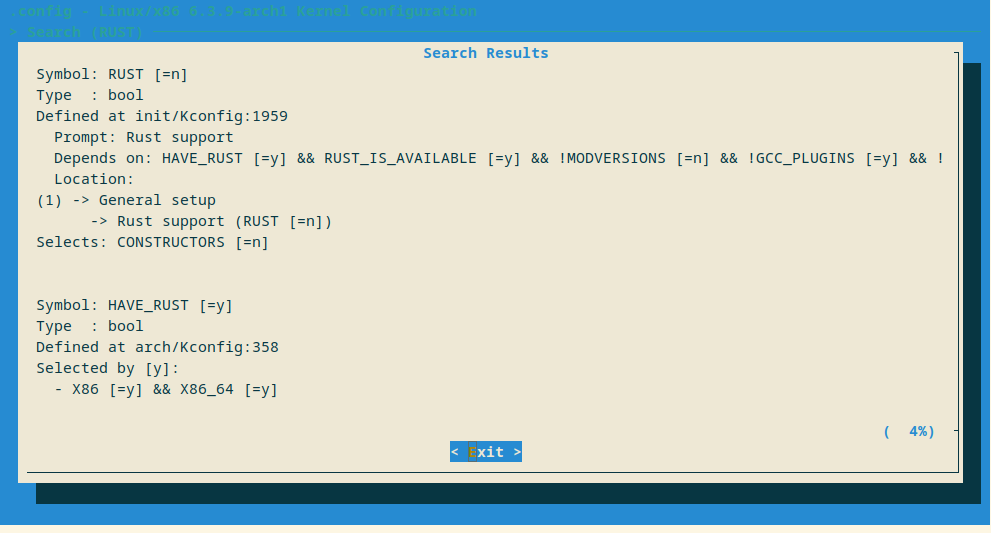
\includegraphics[height=0.75\textheight]{img/make-menuconfig.png}
  \note[item]{The Linux kernel has automatic config variables}
  \note[item]{The Rust support just gets disabled if we have conflicting options}
  \note[item]{\texttt{HAVE\_RUST} is just to \emph{disable} Rust support if everything else would be here}
\end{frame}


\begin{frame}[c,fragile]{What did we learn?}
  \small
\begin{itemize}
\item Rust support needs to compile the kernel with clang/LLVM
\item The kernel only attempts to load modules which have the same version magic
\item It needs a specific \emph{stable} Rust version {\footnotesize(since it uses the
\texttt{RUSTC\_BOOTSTRAP=1} trick to enable unstable features on stable compilers)}
\item The module interface is (of course) still in flux
\item The kernel has automatic configuration variables which detect if stuff can be enabled (\texttt{CONFIG\_RUST\_IS\_AVAILABLE})
\item Actual Rust support depends on a combination of multiple variables
\end{itemize}
\end{frame}

\subsection{January 2023 — Compiling our own kernel}

\begin{frame}[c,fragile]{Building our own kernel}
  \begin{itemize}
    \item The ArchLinux kernel doesn't support Rust modules
    \item I want to have a bootable / useable kernel \rightarrow{} take the
      ArchLinux kernel as base and only do minimal changes
    \item Alternative: Just use the Rust-for-Linux kernel
  \end{itemize}
\end{frame}

\begin{frame}[c,fragile]{Building our own kernel}
  \begin{itemize}
    \item Create https://aur.archlinux.org/packages/linux-rust
    \item Take the ArchLinux kernel package
    \item Run \texttt{make menuconfig}
    \item Enhance the build process with Rust specific stuff
    \item Build kernel, reboot, profit\footnote{Of course this needed some iterations in the build process}
  \end{itemize}
\end{frame}

\begin{frame}[c,fragile]{First sucesses!}
  \begin{minted}[fontsize=\small,breaklines]{bash}
$ make KDIR=~/projects/archpkg/linux-rust/src/archlinux-linux LLVM=1
$ sudo insmod rust_out_of_tree.ko
# dmesg output
[  451.297415] rust_out_of_tree: loading out-of-tree module taints kernel.
[  451.297460] rust_out_of_tree: module verification failed: signature and/or required key missing - tainting kernel
[  451.297724] rust_out_of_tree: Rust out-of-tree sample (init)

  \end{minted}
\end{frame}

\begin{frame}{First sucesses!}
  \centering
  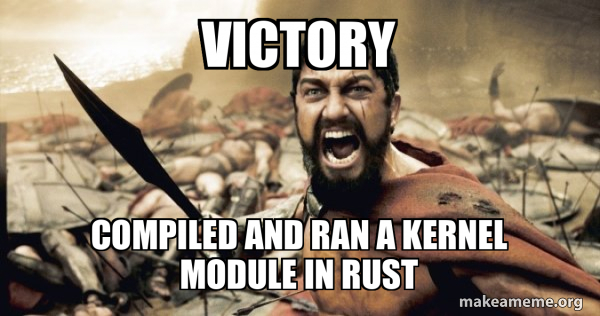
\includegraphics[width=0.9\textwidth]{img/victory-compiled-and-loaded-kernel-module.jpg}
\end{frame}

\begin{frame}[c,fragile]{A small issue...}
  \begin{itemize}
    \item Did you notice our workaround?
      \pause
    \item Right: \texttt{KDIR=\textasciitilde/projects/archpkg/linux-rust/src/archlinux-linux}
    \item This meens we need the sources of our kernel build around. Not nice
      if we want to enable people to install it via package manager
  \end{itemize}
\end{frame}

\begin{frame}[c]{Remember build metadata?}
  \begin{columns}[c]
    \begin{column}{0.5\textwidth}
      
\includegraphics[width=\textwidth]{img/tux-trying-to-remember-what-he-read-in-the-readme.png}
    \end{column}
    \begin{column}{0.5\textwidth}
      \begin{itemize}
        \item Remember the quote about build metadata in the readme?
        \item Let's try to package this correctly!\footnote{The build metadata goes in the linux-rust-headers package. The name is slightly missleading, because it contains various other build artifacts}
      \end{itemize}
    \end{column}
  \end{columns}
\end{frame}

\begin{frame}[c]{Just follow the errors}
My strategy:
  \begin{itemize}
    \item Try to build the out-of-tree module
    \item Check the errors
    \item Add files to the metadata which should fix the issue
    \item \texttt{makepkg --repackage -f} is our friend
  \end{itemize}
\end{frame}

\begin{frame}[c,fragile]{First error: target.json}
  \begin{minted}[fontsize=\small]{text}
rust-out-of-tree-module (git)-[main] % make LLVM=1
make -C /lib/modules/`uname -r`/build M=$PWD
make[1]: Entering directory '/usr/lib/modules/6.1.5-arch2-1-rust/build'
  RUSTC [M] ~/projects/github/Rust-for-Linux/rust-out-of-tree-module/rust_out_of_tree.o
error: target file "./rust/target.json" does not exist
  \end{minted}

  \rightarrow{} Let's add \texttt{install -Dt "\$builddir/rust" -m644 scripts/target.json}
\end{frame}

\begin{frame}[c,fragile]{Next error: core library}
  \begin{minted}[fontsize=\small]{text}
make -C /lib/modules/`uname -r`/build M=$PWD
make[1]: Entering directory '/usr/lib/modules/6.1.5-arch2-1-rust/build'
  RUSTC [M] ~/projects/github/Rust-for-Linux/rust-out-of-tree-module/rust_out_of_tree.o
error[E0463]: can't find crate for `core`
  |
  = note: the `target` target may not be installed
  = help: consider downloading the target with `rustup target add target`
  = help: consider building the standard library from source with `cargo build -Zbuild-std`

  \end{minted}

  \rightarrow{} Let's just add everything from \texttt{rust/}!\footnote{This decision happened after several iterations...}
\end{frame}

\begin{frame}[c,fragile]{Next error: Rust version}
  \begin{minted}[fontsize=\small,breaklines]{text}
error[E0514]: found crate `core` compiled by an incompatible version of rustc
  = note: the following crate versions were found:
          crate `core` compiled by rustc 1.62.0 (a8314ef7d 2022-06-27): /usr/lib/modules/6.1.5-arch2-1-rust/build/rust/libcore.rmeta
  = help: please recompile that crate using this compiler (rustc 1.66.0 (69f9c33d7 2022-12-12)) (consider running `cargo clean` first)
  \end{minted}
  \rightarrow{} We need to put \texttt{rust-toolchain} file into \texttt{/usr/lib/modules/...}, not the out-of-tree module folder!
\end{frame}

\begin{frame}[c,fragile]{Target tripple what?}
  \begin{minted}[fontsize=\small,breaklines]{text}
make -C /lib/modules/`uname -r`/build M=$PWD
make[1]: Entering directory '/usr/lib/modules/6.1.5-arch2-1-rust/build'
  RUSTC [M] /home/roughl/projects/github/Rust-for-Linux/rust-out-of-tree-module/rust_out_of_tree.o
error[E0461]: couldn't find crate `core` with expected target triple target-12809083303779448358
  |
  = note: the following crate versions were found:
          crate `core`, target triple target-3911737072772191946: /usr/lib/modules/6.1.5-arch2-1-rust/build/rust/libcore.rmeta
  \end{minted}
\end{frame}

\begin{frame}[c,fragile]{Target tripple what?}
  \begin{itemize}
    \item WAT?
    \item Target tripples define for what you want to compile
      (\texttt{x86\_64-unknown-linux-gnu} for example)
    \item What was that strange number? Don't we have a custom
      \texttt{target.json} anyway?
  \end{itemize}
\end{frame}

\begin{frame}[c]{What did we learn? (part 2)}
  \small
  \begin{itemize}
    \item Building our own workable kernel was surprisingly easy!
    \item Packaging the correct build metadata not
    \item \texttt{target.json} is used to describe the kernel environement to
      the Rust compiler
    \item The kernel uses it's own Rust library (mostly std libcore, but with
      custom liballoc for example)
    \item out-of-tree module builds get executed in the context of the build
      metadata and are passed the directory of the module.
  \end{itemize}
\end{frame}

\subsection{June 2023 — Packing the correct metadata}

\begin{frame}[c]{Motivation}
  \begin{itemize}
    \item I did update my kernel a few times to keep it up to date and checked
      if anything changed with Linux 6.2\footnote{Here I needed to change back
      the changes we made to the out-of-tree module
      \url{https://github.com/Rust-for-Linux/rust-out-of-tree-module/pull/5}}
    \item I did propose to do this talk
    \item I had some nice interactions with Miguel Ojeda from the
      Rust-for-Linux project!
  \end{itemize}
\end{frame}

\begin{frame}[c]{What I learned growing up with C++/Rust}
  \begin{quote}
    \centering
    Never blame the compiler for an issue you have!
  \end{quote}
  \pause \centering 
\includegraphics[width=0.75\textwidth]{img/one-does-not-simply-blame-the-compiler.jpg}
\end{frame}

\begin{frame}[c]{It was the compiler...}
  \begin{itemize}
    \item For custom \texttt{target.json} the Rust compiler uses a hash to
      assert that the target it the same (the strange number)
    \item The Rust compiler decided (probably as a quick hack?) to use the \emph{path} instead of the \emph{content} of the \texttt{target.json} to calculate this hash! This was fixed in Rustr 1.63.0\footnote{\url{https://github.com/rust-lang/rust/pull/98225/}}
      \pause\item But we need to use 1.62.0\pause, right?
  \end{itemize}
\end{frame}

\begin{frame}[c,fragile]{Compiling with 1.63.0}
  Wrong! We only get some minor warnings in the output:
\begin{minted}[fontsize=\small]{text}
*** Rust compiler 'rustc' is too new. This may or may not work.
***   Your version:     1.63.0
***   Expected version: 1.62.0
warning: the feature `nll` has been stable since 1.63.0 and no longer requires an attribute to enable
   --> rust/alloc/lib.rs:170:12
    |
170 | #![feature(nll)] // Not necessary, but here to test the `nll` feature.
    |            ^^^
    |
    = note: `#[warn(stable_features)]` on by default
\end{minted}
  \note{Remember: The Linux kernel uses unstable features on a stable release!}
\end{frame}

\begin{frame}[c]{Getting the necessary build metadata}
  \begin{itemize}
    \item \texttt{rust/target.json} the custom target description
    \item \texttt{rust/*.rmeta} the compiled rust libraries
    \item \texttt{rust/*.so} the pre-compiled procedural macros
    \item \texttt{rust-toolchain} such that we use the same Rust compiler
      version that was used to compile the kernel
  \end{itemize}
\end{frame}

\begin{frame}[c]{What did we learn? (part 3)}
  \begin{itemize}
    \item Sometimes it \emph{is} the compiler
    \item Just upgrading one version of the Rust compiler was safe (A
      stabilized feature should probably not change from the last release)
  \end{itemize}
\end{frame}

\subsection{June 2023 — There and Back Again}

\begin{frame}[c]{Updating to 6.3}
  \begin{itemize}
    \item We did it
    \item We can compile out-of-tree modules!
    \item Now we can just update and play around with new features that land for Rust modules!
    \pause\item Right?
  \end{itemize}
\end{frame}

\begin{frame}[c,fragile]{Updating to 6.3}
  Wrong!
\begin{minted}[fontsize=\small,breaklines]{text}
rust-out-of-tree-module (git)-[main] % make LLVM=1
make -C /lib/modules/6.3.8-arch1-1-rust/build M=$PWD
 RUSTC [M] rust-out-of-tree-module/rust_out_of_tree.o
error: could not write output to rust_out_of_tree.rust_out_of_tree.ad9c6f77-cgu.0.rcgu.o: Permission denied

error: aborting due to previous error
\end{minted}
\end{frame}

\begin{frame}[c]{Updating to 6.3}
  Asking on the Rust-for-Linux
  chat\footnote{\url{https://rust-for-linux.zulipchat.com/\#narrow/stream/291565-Help/topic/Out.20of.20tree.20module.20for.20mainline.20kernel}}

  \texttt{rustc} writes temporary files to the current directory\footnote{Which is in \texttt{/lib/modules/...} for the module build}, even if we specify
  with \texttt{--emit} where we want our output file.

  We need to pass \texttt{--out-dir}
\end{frame}

\begin{frame}[c,fragile]{Updating to 6.3}
\begin{minted}[fontsize=\small,breaklines]{diff}
diff --git a/scripts/Makefile.build b/scripts/Makefile.build
index 94d67252df4e..261e51c0af59 100644
--- a/scripts/Makefile.build
+++ b/scripts/Makefile.build
@@ -287,7 +287,7 @@ rust_common_cmd = \
        --extern alloc --extern kernel \
        --crate-type rlib -L $(objtree)/rust/ \
        --crate-name $(basename $(notdir $@)) \
-       --emit=dep-info=$(depfile)
+       --out-dir $(dir $@) --emit=dep-info=$(depfile)
\end{minted}
\end{frame}

\begin{frame}[c]{What did we learn? (part 4)}
  \begin{itemize}
    \item Nobody except me cares for out-of-tree Rust kernel modules so far {\Emoji😉}
    \item The Rust-for-Linux community is very helpful!
      {\Emoji🎉}
  \end{itemize}
\end{frame}


\section{Some Outlook}

\begin{frame}[c]{Linux 6.5}
% * Linux 6.5 will get a newer Rust version and will start updating it regularly
\end{frame}

% * There is quite some stuff done using Rust in the Linux kernel very notably Apple M1/M2 GPU support by Asahi Linux


% ----------------------------------------------------------------- %

{
\setbeamertemplate{footline}{}
\pgfdeclareimage[width=\paperwidth]{bg}{background-inverted.pdf}
\usebackgroundtemplate{\pgfuseimage{bg}}
\begin{frame}[standout]
  \begin{centering}
    {\Huge Thank you!}\\
    {\normalsize \url{https://coredump.ch}}\\
    {\normalsize \url{https://renuo.ch/}}\\
  \end{centering}
  {\small Slides: \url{https://github.com/rust-zurichsee/meetups/}}\\
  \vspace{3cm}
\end{frame}
}


\setbeamertemplate{section in toc}[sections numbered]
\pgfdeclareimage[width=\paperwidth]{bg}{background-light.pdf}
\usebackgroundtemplate{\pgfuseimage{bg}}
\appendix
\section{\appendixname}
\frame{\tableofcontents}

\subsection{Appendix}

\begin{frame}[c]{Appendix}
\end{frame}

\end{document}
